\section{HHL Algorithmus}

\subsubsection{Übersicht}

    \begin{frame}
    \frametitle{Übersicht}
        Vergleich klassische zur quanten Version

        \hfil
        \begin{columns}[c]
            \begin{column}{0.6\hsize}\centering
            Klassisch
            $$A \vec{x} = \vec{b}$$
            $$\vec{x} = A^{-1}\vec{b}$$
            \end{column}

            \begin{column}{0.4\hsize}
            Quanten Version
            $$A \ket{x} = \ket{b}$$
            $$\ket{x} = A^{-1}\ket{b}$$
            \end{column}
        \end{columns}

    

    \end{frame}


    \begin{frame}
    \frametitle{Übersicht}

        \hfil

        $A$ kann man auch in der Spektralzerlegung darstellen

        \hfil
        \begin{columns}[c]
            \begin{column}{0.4\hsize}\centering
            $$A = \sum_{i=0}^{2^{n_b}-1} \lambda_i \ket{u_i}\bra{u_i}$$
            $$A^{-1} = \sum_{i=0}^{2^{n_b}-1} \lambda_i^{-1} \ket{u_i}\bra{u_i}$$
            \end{column}

            \begin{column}{0.6\hsize}
            \begin{itemize}
            \item   $\lambda_i$ sind Eigenwerte von A
            \item   $\ket{u_i}$ sind Eigenvektoren von A
            \end{itemize}
 
            \end{column}
        \end{columns}

        \hfil

        \hfil

        $\vec{b}$ kann in der Eigenbasis von $A$ dargestellt werden 

        \hfil

        \begin{columns}[c]
            \begin{column}{0.4\hsize}\centering
            $$\ket{b} = \sum_{j=0}^{2^{n_b}-1} b_j\ket{u_j}$$
            \end{column}
            \begin{column}{0.6\hsize}
            \begin{itemize}
            \item   $b_i$ sind die koeffizienten von $\vec{b}$
            \item   $\ket{u_i}$ sind Eigenvektoren von A
            \end{itemize}
 
            \end{column}
        \end{columns}



   \end{frame}

    \begin{frame}
    \frametitle{Übersicht}

        Setzen wir nun alles ein:

        \hfil
        $$\ket{x} = A^{-1} \ket{b} = \left( \sum_{i=0}^{2^{n_b}-1} \lambda_i^{-1} \ket{u_i}\bra{u_i} \right) \left( \sum_{j=0}^{2^{n_b}-1} b_j\ket{u_j} \right)$$
        $$\ket{x}= \sum_{i=0}^{2^{n_b}-1} \sum_{j=0}^{2^{n_b}-1} \lambda_i^{-1} \ket{u_i}\bra{u_i} b_j\ket{u_j}$$
        $$\ket{x}= \sum_{i=0}^{2^{n_b}-1} \sum_{j=0}^{2^{n_b}-1} \lambda_i^{-1} b_j\ket{u_i}\braket{u_i| u_j}$$
        $$\ket{x} = \sum_{i=0}^{2^{n_b}-1} \sum_{j=0}^{2^{n_b}-1} \lambda_i^{-1} b_j\ket{u_i}\delta_{ij}$$

    \end{frame}


    \begin{frame}
    \frametitle{Übersicht}
        Setzen wir nun alles ein (Fort.):

        \hfil
        $$\ket{x} = \sum_{i=0}^{2^{n_b}-1} \sum_{j=0}^{2^{n_b}-1} \lambda_i^{-1} b_j\ket{u_i}\delta_{ij}$$
        $$\ket{x} =  A^{-1} \ket{b} = \sum_{i=0}^{2^{n_b}-1} \lambda_i^{-1} b_j\ket{u_j}$$
        $$\ket{x} =  A^{-1} \ket{b} = \sum_{i=0}^{2^{n_b}-1} \lambda_i^{-1} b_j\ket{u_j}$$

    \end{frame}

    \begin{frame}
    \frametitle{Übersicht}
        \begin{enumerate}
            \item Ermittle die Eigenwerte und Eigenvektoren von $A$
            \item bilde $\ket{b}$ in Eigenbasis $A$ ab
            \item  Invertiert Eigenwerte
            \item lies das Ergebnis $\ket{x}$ aus
        \end{enumerate}
    \end{frame}

\subsubsection{Der Algorithmus}

    \begin{frame}
    \frametitle{Der Algorithmus}

        \textbf{Ablauf}
        \begin{enumerate}
            \item State Preparation
            \begin{itemize}
                \item Enkodiere Vektor und Matrix in Quanten Computer
            \end{itemize}
            \item Quantum Phase Estimation
            \begin{itemize}
                \item ermittle Eigenwerte und Eigenvektoren 
                \item bilde $\ket{b}$ in Eigenbasis $A$ ab
            \end{itemize}
            \item Ancilla Bit Rotation 
            \begin{itemize}
                \item  Invertiert Eigenwerte
            \end{itemize}
            \item Inverse Quantum Phase Estimation
             \begin{itemize}
                \item löst verschränkte Qubits auf
            \end{itemize}
            
            \item Messung
             \begin{itemize}
                \item liest das Ergebnis $\ket{x}$ aus
            \end{itemize}
 
        \end{enumerate}

    \end{frame}

    \begin{frame}
    \frametitle{Quantum Circuit}
    \begin{center}
    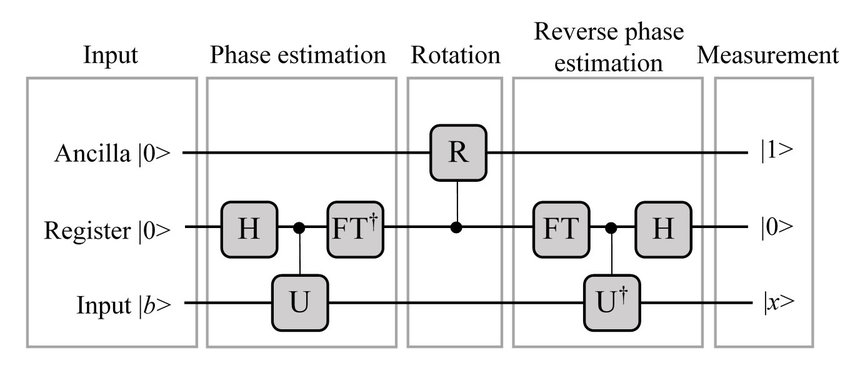
\includegraphics[width=10cm]{img/hhl_circuit.jpg}
    \end{center}

    \begin{enumerate}
        \item Ancilla (Helfer): a-register
        \begin{itemize}
            \item Indikator qubit - zeigt an ob Zustände verschränkt sind
        \end{itemize}

        \item Register: c-register
        \begin{itemize}
            \item beinhaltet später die eigenwerte
        \end{itemize}
        
        \item Input: b-register 
        \begin{itemize}
            \item beinhaltet den Vektor $\vec{b}$
        \end{itemize}
        
    \end{enumerate}
   \end{frame}

\begin{frame}
    \frametitle{Quantum Circuit}
    \hfil

    Wo befindet sich die Matrix $A$?
    \begin{center}
    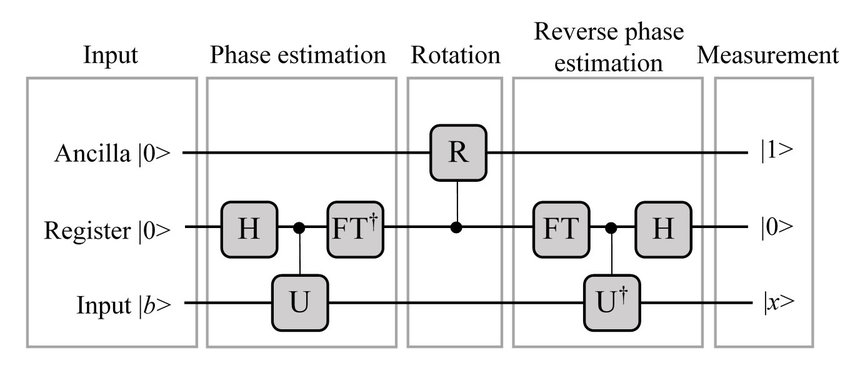
\includegraphics[width=10cm]{img/hhl_circuit.jpg}
    \end{center}

    \hfil
    Wir als Unitary (Einheitsmatrix) in die Phase Estimation enkodiert.
    $$U = e^{iAt}$$
\end{frame}

\begin{frame}
    \frametitle{Quantum Circuit}
    \begin{center}
    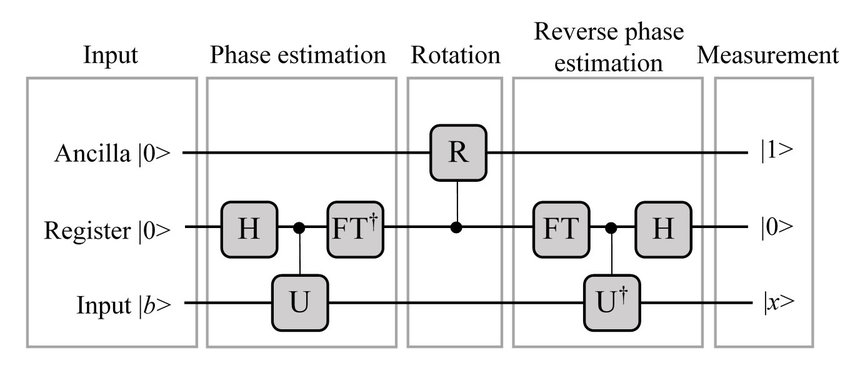
\includegraphics[width=10cm]{img/hhl_circuit.jpg}
    \end{center}

    Wir starten im 0 Zustand
    $$\ket{\Psi_0} = \ket{0}_b\ \ket{0}_c\ \ket{0}_a$$


\end{frame}


\begin{frame}
    \frametitle{State Preparation}
    
    \hfil

    Nun werden wir $\vec{b}$ als Quantenzustand $\ket{b}$ kodieren, 
    indem wir die Elementen von $\vec{b}$ den Amplituden von $\ket{b}$ zuordnen.

    $$\vec{b}=\begin{pmatrix} b_0 \\ b_1 \\ ... \\b_n \end{pmatrix}
        \Leftrightarrow b_0 \ket{0} + b_1 \ket{1} + ... + b_n \ket{n} = \ket{b}$$

    \hfil

\end{frame}
\begin{frame}
    \frametitle{State Preparation}
    \begin{center}
    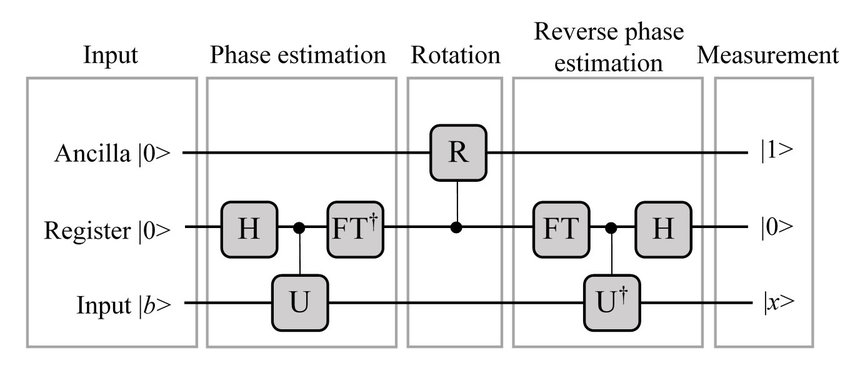
\includegraphics[width=10cm]{img/hhl_circuit.jpg}
    \end{center}

    Dann erhalten wir:
    $$\ket{\Psi_1} = \ket{b}_b\ \ket{0...0}_c\ \ket{0}_a$$


\end{frame}

\begin{frame}
    \frametitle{Quantum Phase Estimation}
    \begin{center}
    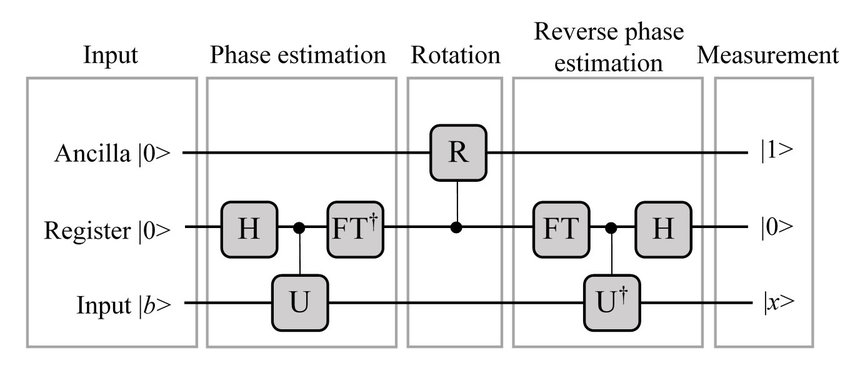
\includegraphics[width=10cm]{img/hhl_circuit.jpg}
    \end{center}

    Wir wenden QPE an, um die Eigenwerte von A zu erhalten.
    Dann erhalten wir:
    $$\ket{\Psi_2} = \ket{b}_b \ket{\widetilde{\lambda_j}}_c\ket{0}_a$$


\end{frame}


\begin{frame}
    \frametitle{Ancilla Roation - Eigenwerte invertieren}

    Rotation des Ancilla Bits
    \begin{itemize}
        \item Ancilla-Bit $\ket{0}_a$ wird anhand der Eigenwerte $\ket{ \widetilde{\lambda}_j}$ rotiert
        \item hat eine Fehlerwahrscheinlichkeit, da Operation nicht unitär 
    \end{itemize}

    \hfil

    Ancilla-Qubit wird gemessen und kollabiert zu
    \begin{enumerate}
        \item $\ket{0}$: Ergebnis wird verworfen, Berechnung wird wiederholt
            \begin{itemize}
            \item wir haben verschränkte Qubits
            \item dies wird Amplitudenverstärkung genannt (wie Grover)
            \end{itemize}
        \item $\ket{1}$: Ergebnis wird akzeptiert
    \end{enumerate}

\end{frame}

\begin{frame}
    \frametitle{Ancilla Roation - Eigenwerte invertieren}
    Rotation des Ancilla Bits
$$\ket{\Psi_3} = \sum_{j=0}^{2^{n_b}-1} b_j \ket{u}_j  \ket{\widetilde{\lambda}_j} \left( \sqrt{1-\frac{C^2}{\widetilde{\lambda}_j^2}} \ket{0}_a + \frac{C}{\widetilde{\lambda}_j} \ket{1}_a\right)$$

    $$\ket{\Psi_3} = \ket{b}_b \ket{\widetilde{\lambda_j}}_c\ket{??}_a$$

    \hfil

    Gehen wir davon aus, dass unsere Ancilla-Qubit auf $\ket{1}$ kollabiert.
$$\ket{\Psi_3} = \frac {1} {\sqrt{\sum_{j=0}^{2^{n_b}-1} | \frac{b_jC} {\widetilde{\lambda}_j}|^2}}
\sum_{j=0}^{2^{n_b}-1} b_j \ket{u_j}  \ket{\widetilde{\lambda}_j} \frac{C}{\widetilde{\lambda}_j} \ket{1}_a$$

    $$\ket{\Psi_3} = \ket{b}_b \ket{\widetilde{\lambda_j}}_c \widetilde{\lambda^{-1}} \ket{1}_a$$

\end{frame}


\begin{frame}
    \frametitle{Ancilla Roation - Eigenwerte invertieren}
    \begin{center}
    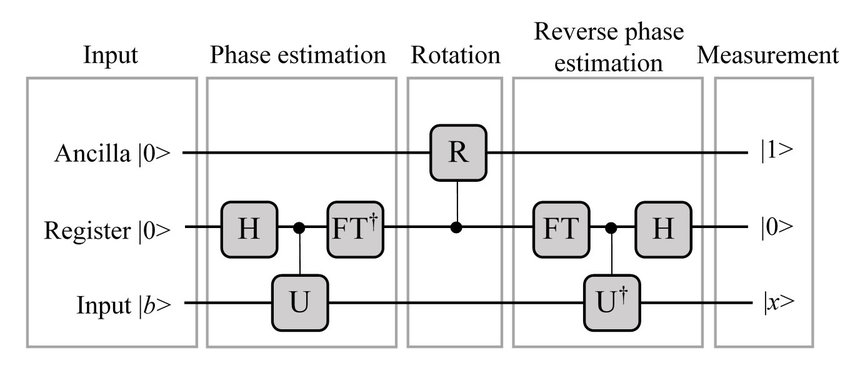
\includegraphics[width=10cm]{img/hhl_circuit.jpg}
    \end{center}

    Dann erhalten wir:
    $$\ket{\Psi_3} = \ket{b}_b \ket{\widetilde{\lambda_j}}_c \widetilde{\lambda^{-1}} \ket{1}_a$$


\end{frame}

\begin{frame}
    \frametitle{Ancilla Roation - Eigenwerte invertieren}

    Uns fällt auf, dass wir schon sehr nah an unserem Ergebnis sind
    \begin{columns}[c]
        \begin{column}{0.5\hsize}\centering
        $$\ket{\Psi_3} = \ket{b}_b \ket{\widetilde{\lambda_j}}_c \widetilde{\lambda^{-1}} \ket{1}_a$$
        \end{column}
        \begin{column}{0.5\hsize}
        $$\ket{x} =  A^{-1} \ket{b} = \sum_{i=0}^{2^{n_b}-1} \lambda_i^{-1} b_i\ket{u_i}$$
        \end{column}
    \end{columns}

    \hfil

    \begin{itemize}
        \item Eigenwerte sind invertiert.
        \item aber b-Register mit c-Register verschränkt, $\ket{\widetilde{\lambda}_j}$.
        \item müssen den Zustand auflösen (alle bisherigen Schritte rückgäng machen)
    \end{itemize}



\end{frame}


\begin{frame}

    \frametitle{Inverse Quantum Phase Estimation}
    \begin{center}
    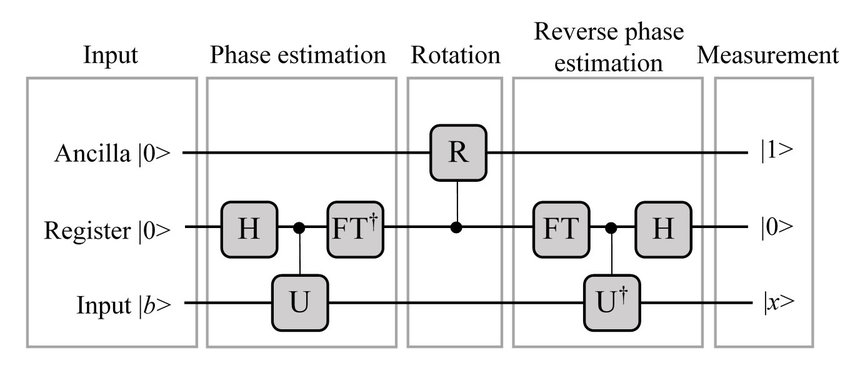
\includegraphics[width=10cm]{img/hhl_circuit.jpg}
    \end{center}

    Dann erhalten wir:

    $$\ket{\Psi_4} = \ket{x}_b \ket{0...0}_c\ket{1}_a$$


\end{frame}


\begin{frame}
    \frametitle{Measurment}
    
    \begin{itemize}
        \item $\ket{x}_b$ kann nicht ausgelesen werden, da nur $log_2(n)$ Einträge 
        \item können Erwartungswert durch Messungen $M$ ermitteln
        $$ E(x) := \bra{x}M\ket{x} $$

    \end{itemize}
\end{frame}

\begin{frame}
    \frametitle{Measurment}
    \begin{center}
    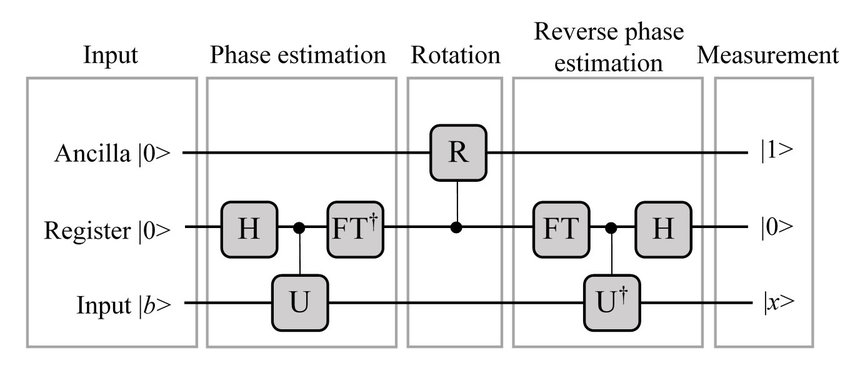
\includegraphics[width=10cm]{img/hhl_circuit.jpg}
    \end{center}

    
    Dann erhalten wir:
        $$\ket{x} \Rightarrow E(x) = \bra{x}M\ket{x} $$


\end{frame}
